% Chapter Template

\chapter{FDTD - Two-Dimensional Scenario} % Main chapter title

\label{Chapter3} % Change X to a consecutive number; for referencing this chapter elsewhere, use \ref{ChapterX}

%----------------------------------------------------------------------------------------
%	SECTION 1
%----------------------------------------------------------------------------------------

Now that we completed the one-dimensional scenario, the following is going to be much easier, as we are going to use the same logic for the most part. For the interest of saving time, redundant information that was covered previously is going to be omitted.

\section{2D Discretization}

In the previous chapter we mentioned the different transverse modes available for electromagnetic waves, but did not go too much in depth as they were not too relevant in that scenario. In a one-dimensional case, it does not matter much which axis we pick for which field, so long as they are perpendicular to which other (something that axes do by default). In the two-dimensional scenario however, the mode we choose is going to dictate our curls. 

\subsection{2D Transverse Modes}

For the two-dimensional scenarios, choosing a transverse mode means that the field we chose will have no field in the direction of propagation, meaning the $z$ axis in our case. That means that any vector moving along that axis will have a value of zero for that field. However, the other field can only have values alongside that direction, meaning that it will be zero for the $x$ and $y$ axis instead. More specifically, each mode features the following field vectors:

\begin{itemize}
	\item \textbf{TE mode} - \space $\vec{E_x},\; \vec{E_y},\; \vec{H_z}$
	\item \textbf{TM mode} - \space $\vec{E_z},\; \vec{H_x},\; \vec{H_y}$
\end{itemize}

While each mode will have us working with different vectors, the process is roughly the same. For our scenario, we will use TE mode, meaning that $\vec{E_z}, \vec{H_x}, \vec{H_y} = 0$.

\subsection{2D TE Electromagnetic Curls}

Similar to the one-dimensional scenario, each vector will have a curl around it, such as the $H_z$ vector in figure \ref{fig:fdtd2dHz}:

\begin{figure}[h!]
	\centering
	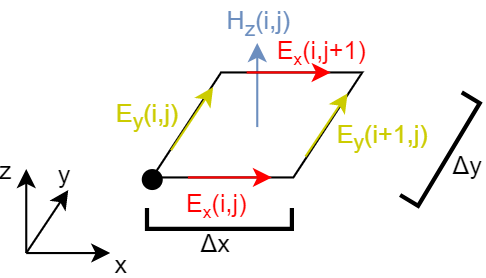
\includegraphics[scale=0.6]{Figures/fdtd2dHz}
	\decoRule
	\caption[2D TE Mode - $H_z$ vector curl]{The curl around the magnetic field vector $H_z$.}
	\label{fig:fdtd2dHz}
\end{figure}

Using a similar indexing scheme as we did previously, we have:

\begin{equation}
	\label{eqn:indexing2DElectric}
	E_{i,j} = E(i \cdot \Delta x , j \cdot \Delta y)
\end{equation}

\begin{multline}
	\label{eqn:2dHzCurl1}
	\oint \vec{E} \cdot d\vec{s} = - \frac{d}{dt} \iint \mu \cdot \vec{H} \cdot d\vec{A} \\
	\Rightarrow E_x(i,j) \cdot \Delta x - E_x(i,j+1) \cdot \Delta x + E_y(i+1,j) \cdot \Delta y - E_y(i,j) \cdot \Delta y \\ = -\frac{d}{dt}(\mu \cdot H_z(i,j) \cdot \Delta x \cdot \Delta y)
\end{multline}

which leads to

\begin{equation}
	\label{eqn:2dHzCurl2}
	\frac{d}{dt} H_z(i,j) = -\frac{1}{\mu} \cdot (\frac{E_x(i,j) - E_x(i,j+1)}{\Delta y} + \frac{E_y(i+1,j)- E_y(i,j)}{\Delta x})
\end{equation}

If we have a uniform mesh size, meaning that $\Delta x = \Delta y =  \Delta z = \Delta s$, we can simplify equation \ref{eqn:2dHzCurl2} to:

\begin{equation}
	\label{eqn:2dHzCurl3}
	\frac{d}{dt} H_z(i,j) = -\frac{1}{\mu \cdot \Delta s} \cdot ((E_x(i,j) - E_x(i,j+1) + E_y(i+1,j)- E_y(i,j))
\end{equation}

For the left hand side, we know that:

\begin{equation}
	\label{eqn:2dHzCurl4}
	\frac{d}{dt} H_z(i,j) = \frac{H_z^{new}(i,j) - H_z^{prev}(i,j)}{\Delta t}
\end{equation}

By combining equations \ref{eqn:2dHzCurl3} and \ref{eqn:2dHzCurl4}, we get our update equation for the magnetic field vector $H_z$:

\begin{multline}
	\label{eqn:2dHzCurlFinal}
	H_z^{new}(i,j) =  H_z^{prev}(i,j) -\frac{\Delta t}{\mu \cdot \Delta s} \cdot \\ (E_x(i,j) - E_x(i,j+1) + E_y(i+1,j)- E_y(i,j))
\end{multline}

For the electric vectors $E_x$ and $E_y$, the equations and curls are going to be roughly the same as the ones for the one-dimensional scenario. The curl for $E_x$ can be seen in Figure \ref{fig:fdtd2dEx}:

\begin{figure}[h!]
	\centering
	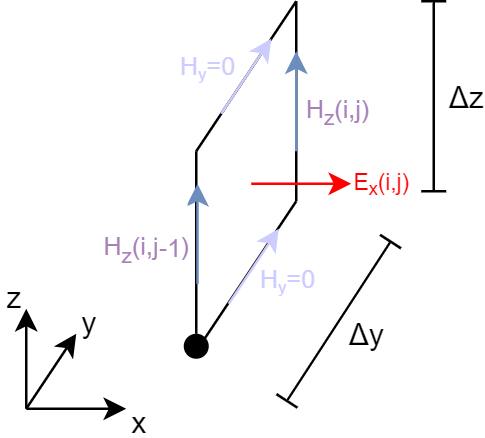
\includegraphics[scale=0.6]{Figures/fdtd2dEx}
	\decoRule
	\caption[2D TE Mode - $E_x$ vector curl]{The curl around the electric field vector $E_x$.}
	\label{fig:fdtd2dEx}
\end{figure}

resulting in the following update equation:

\begin{equation}
	\label{eqn:2dExCurlFinal}
	E_x^{new}(i,j) =  E_x^{prev}(i,j) + \frac{\Delta t}{\epsilon \cdot \Delta s} \cdot (H_z(i,j) - H_z(i,j-1))
\end{equation}

In a similar fashion, the curls for $E_y$ will be as follows (Figure \ref{fig:fdtd2dEy}),

\begin{figure}[h!]
	\centering
	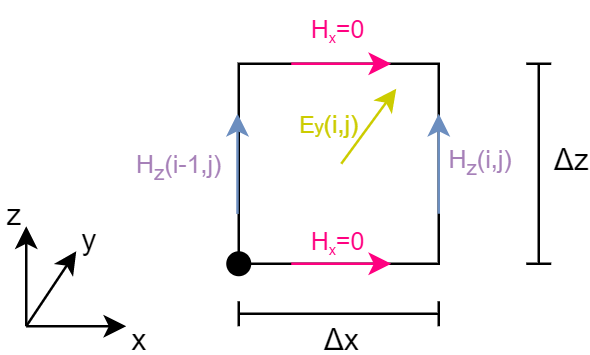
\includegraphics[scale=0.6]{Figures/fdtd2dEy}
	\decoRule
	\caption[2D TE Mode - $E_y$ vector curl]{The curl around the electric field vector $E_y$.}
	\label{fig:fdtd2dEy}
\end{figure}

with a fairly similar equation (note the signs):

\begin{equation}
	\label{eqn:2dEyCurlFinal}
	E_y^{new}(i,j) =  E_y^{prev}(i,j) - \frac{\Delta t}{\epsilon \cdot \Delta s} \cdot (H_z(i,j) - H_z(i-1,j))
\end{equation}

We can now proceed to the code implementation.

\section{C++ Implementation}

Starting off with our imports, we are going to ignore the ones we already discussed. We have however, added three new imports:

\begin{minted}[breaklines,frame=single,fontsize=\footnotesize]{c++}
#include <io.h>
#include <fstream>
\end{minted}

For the two dimensional scenario, we are going to change the way we visualize our data. The end result will be an animation that shows us how the waves propagate in real time. We will get deeper into it once we discuss data visualization, but for now all we need to know is that the output of the two-dimensional implementation is going to be CSV files. Our packages above help us with that:

\begin{itemize}
	\item \textbf{fstream}\textsuperscript{\cite{fstream}} - Input output stream operations for files. Allows us to create and modify them.
	\item \textbf{io.h}\textsuperscript{\cite{io.h}} - Header file used by \textbf{fstream} among other packages.
\end{itemize}

We are also going to introduce two new methods to write our electromagnetic data into files:

\begin{minted}[breaklines,frame=single,fontsize=\footnotesize]{c++}
void writeEDataToCsvFile(string filename, vector<vector<double>> Ex, vector<vector<double>> Ey){
	
	//	"x","y",Ex,Ey
	//	0,0,Ex[x,y],Ey[x,y]
	
	ofstream csvFile(filename);
	csvFile << "x,y,z,Ex,Ey\n";
	
	for (unsigned x = 0; x < Ex[0].size(); x++) {
		for (unsigned y = 0; y < Ex[x].size(); y++) {
			csvFile << to_string(x) + "," + to_string(y) + ",0," + to_string(Ex[x][y]) + "," + to_string(Ey[x][y]) + "\n";
		}
	}
	
	csvFile.close();
}

void writeHDataToCsvFile(string filename, vector<vector<double>> Hz){
	
	//	"x","y",Hz
	//	0,0,Hz[x,y]
	
	ofstream csvFile(filename);
	csvFile << "x,y,z,Hz\n";
	
	for (unsigned x = 0; x < Hz[0].size(); x++) {
		for (unsigned y = 0; y < Ex[x].size(); y++) {
			csvFile << to_string(x) + "," + to_string(y) + ",0," + to_string(Hz[x][y]) + "\n";
		}
	}
	
	csvFile.close();
}
\end{minted}

We will be calling these methods every time we loop, to print a file that contains the respective field's data for that time step. The filename format should be \textit{"X.csv.n"}, where \textit{X} is the field the data is for (E for electric, H for magnetic), while \textit{n} is the time step number. These files are going to get added in the the directory: \mint{c++}{const string filePath = "./Out/";}

We must also make some minor changes to the code to adapt it to a two-dimensional environment. For starters, we need to initialize our vectors as two-dimensional vectors. We also need two vectors for the electric field now, one for the $x$ axis and one for the $y$ axis.

\begin{minted}[breaklines,frame=single,fontsize=\footnotesize]{c++}
vector<vector<double>> Ex(N, vector<double> (N, 0));
vector<vector<double>> Ey(N, vector<double> (N, 0));
vector<vector<double>> Hz(N, vector<double> (N, 0));
\end{minted}

Normally we would also need to add new variables for our deltas:
\begin{minted}[breaklines,frame=single,fontsize=\footnotesize]{c++}
double deltaX = L / N;
double deltaY = L / N;
double deltaZ = L / N;
\end{minted}

Since we have a uniform mesh, meaning all the spatial steps have the same dimensions, we are only going to use one of them (\textit{deltaZ}). In the Appendix (\ref{AppendixA}) we are going to discuss how they can be implemented for unequal time step meshes. For now, since we are only using one of them, our $\Delta t$ will need to be changed to:

\begin{minted}[breaklines,frame=single,fontsize=\footnotesize]{c++}
double deltaT = (deltaZ * sqrt(permitivity*permeability)  * (1/sqrt(2)));
\end{minted}

Another difference is that we are going to apply our Gaussian pulse excitation in the center of the magnetic field this time. Due to the impedance of vacuum, we are going to promptly reduce the magnitude of this excitation, as otherwise we would get electric values that will be far too large.

\begin{minted}[breaklines,frame=single,fontsize=\footnotesize]{c++}
// reducing the magnitude since in free space
Hz[99][99] = exp(-(beta * pow((t - gamma), 2))) * 10e-4;
\end{minted}

Starting from the center will give us a nice symmetric propagation towards the edges. In symmetrical scenarios we can save computation time by splitting the domain into equal parts. It is even more helpful with circular symmetry as we can effectively split it into as many parts as we want, calculate the wave propagation for only one part, then replicate those values for the other parts. This will also be discussed in the Appendix, but for now we will move on with our most basic scenario.

By translating the update equations into code, we get the following in our main loop:

\begin{minted}[breaklines,frame=single,fontsize=\footnotesize]{c++}
for (int i = 0; i < N-1; i++) {
	for (int j = 1; j < N-1; j++) {
		Ex[i][j] = Ex[i][j] + (deltaT / permitivity / deltaZ) * (Hz[i][j] - Hz[i][j-1]);
	}
}

for (int i = 1; i < N-1; i++) {
	for (int j = 0; j < N-1; j++) {
		Ey[i][j] = Ey[i][j] - ((deltaT / permitivity / deltaZ) * (Hz[i][j] - Hz[i-1][j]));
	}
}
writeEDataToCsvFile((filePath + "E/E.csv." + to_string(i)), Ex, Ey);

// loop for values
for (int i = 0; i < N-2; i++) {
	for (int j = 0; j < N-2; j++) {
		Hz[i][j] = Hz[i][j] - ((deltaT / permeability / deltaZ) * (Ex[i][j] - Ex[i][j+1] + Ey[i+1][j] - Ey[i][j]));
	}
}
writeHDataToCsvFile((filePath + "H/H.csv." + to_string(i)), Hz);
\end{minted}

After we are done with each vector field, we can call the respective method to write our data into csv files. For organizational purposes, we will dump the data into separate folders. After waiting for code execution to finish, we will now have two folders with data that is ready to be used for visualization.

\section{Data Visualization}

In order to visualize two-dimensional data in a meaningful manner, we are going to use a helpful open source program called Paraview\textsuperscript{\cite{paraview}}. It allows us to build real time simulations with the data we generated. It is also the reason we chose to name our files the way we did. By using the format \textit{X.csv.n} we can import all of our data as one object. We can do so easily by simply opening Paraview, selecting all of our data, and just dragging and dropping it into the "Pipeline Browser" panel, pictured below (Figure \ref{fig:paraviewFDTD2D1}).

\begin{figure}[h!]
	\centering
	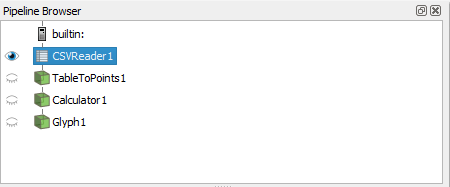
\includegraphics[scale=0.6]{Figures/paraviewFDTD2D1}
	\decoRule
	\caption[2D TE Mode - $E_x$ vector curl]{The curl around the electric field vector $E_x$.}
	\label{fig:paraviewFDTD2D1}
\end{figure}

Having just the data by itself will not do much however. That is why we need to apply filters to the data. They are:

\begin{itemize}
	\item \textbf{Table to Points} - Simply displays the CSV data we got as points.
	\item \textbf{Calculator} - Allows us to manipulate the data and dictate which value goes where.
	\item \textbf{Glyph} - Transforms the data into lines which are better in visualizing vector fields
\end{itemize}

The order is important, as is the fact that each of these filters must be configured properly. For \textbf{Table to Points}, we must define the axes of our data. In our files, we have specified $x$ and $y$, but also $z$, which contains only zeros. We needed to do that since Paraview will not accept an empty value here. It is also helpful to tick \textbf{Axes Grid} under the \textbf{Annotations} category. In the \textbf{Calculator}, we need to add the following formula \mint{java}{iHat*Ex+jHat*Ey} which will unify our point data. Lastly, for the \textbf{Glyph}, we need to use the \textbf{Result} array we got from our \textbf{Calculator} as both \textbf{Orientation} and \textbf{Scaling}. Depending on whether the data is visible or not, we can change the scaling slider until we get what we need. If done correctly, we will get a result similar to Figure \ref{fig:FDTD2DE}.

\begin{figure}[h!]
	\centering
    \begin{subfigure}{.49\textwidth}
    	\centering
    	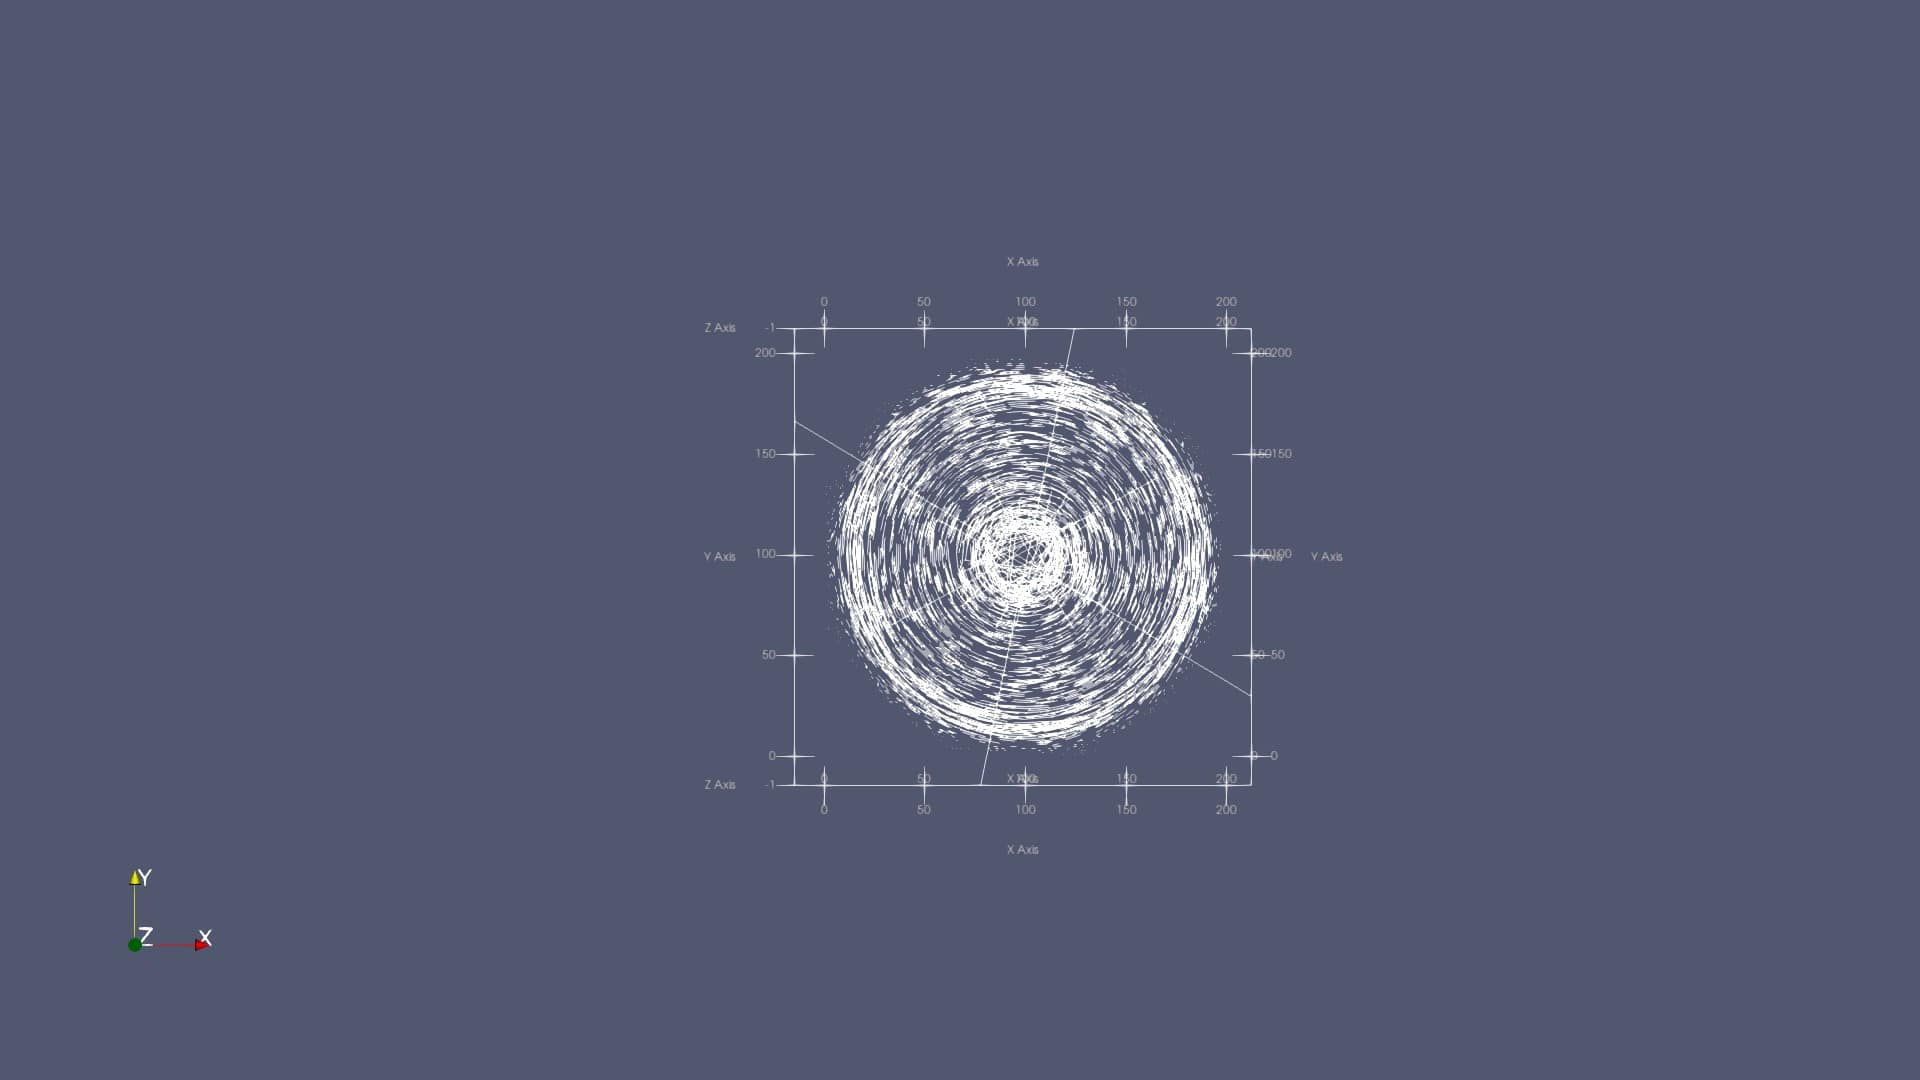
\includegraphics[width=.95\linewidth]{Figures/FDTD2DE1}
    	\caption{t = 200}
    \end{subfigure}
    \begin{subfigure}{.49\textwidth}
    	\centering
    	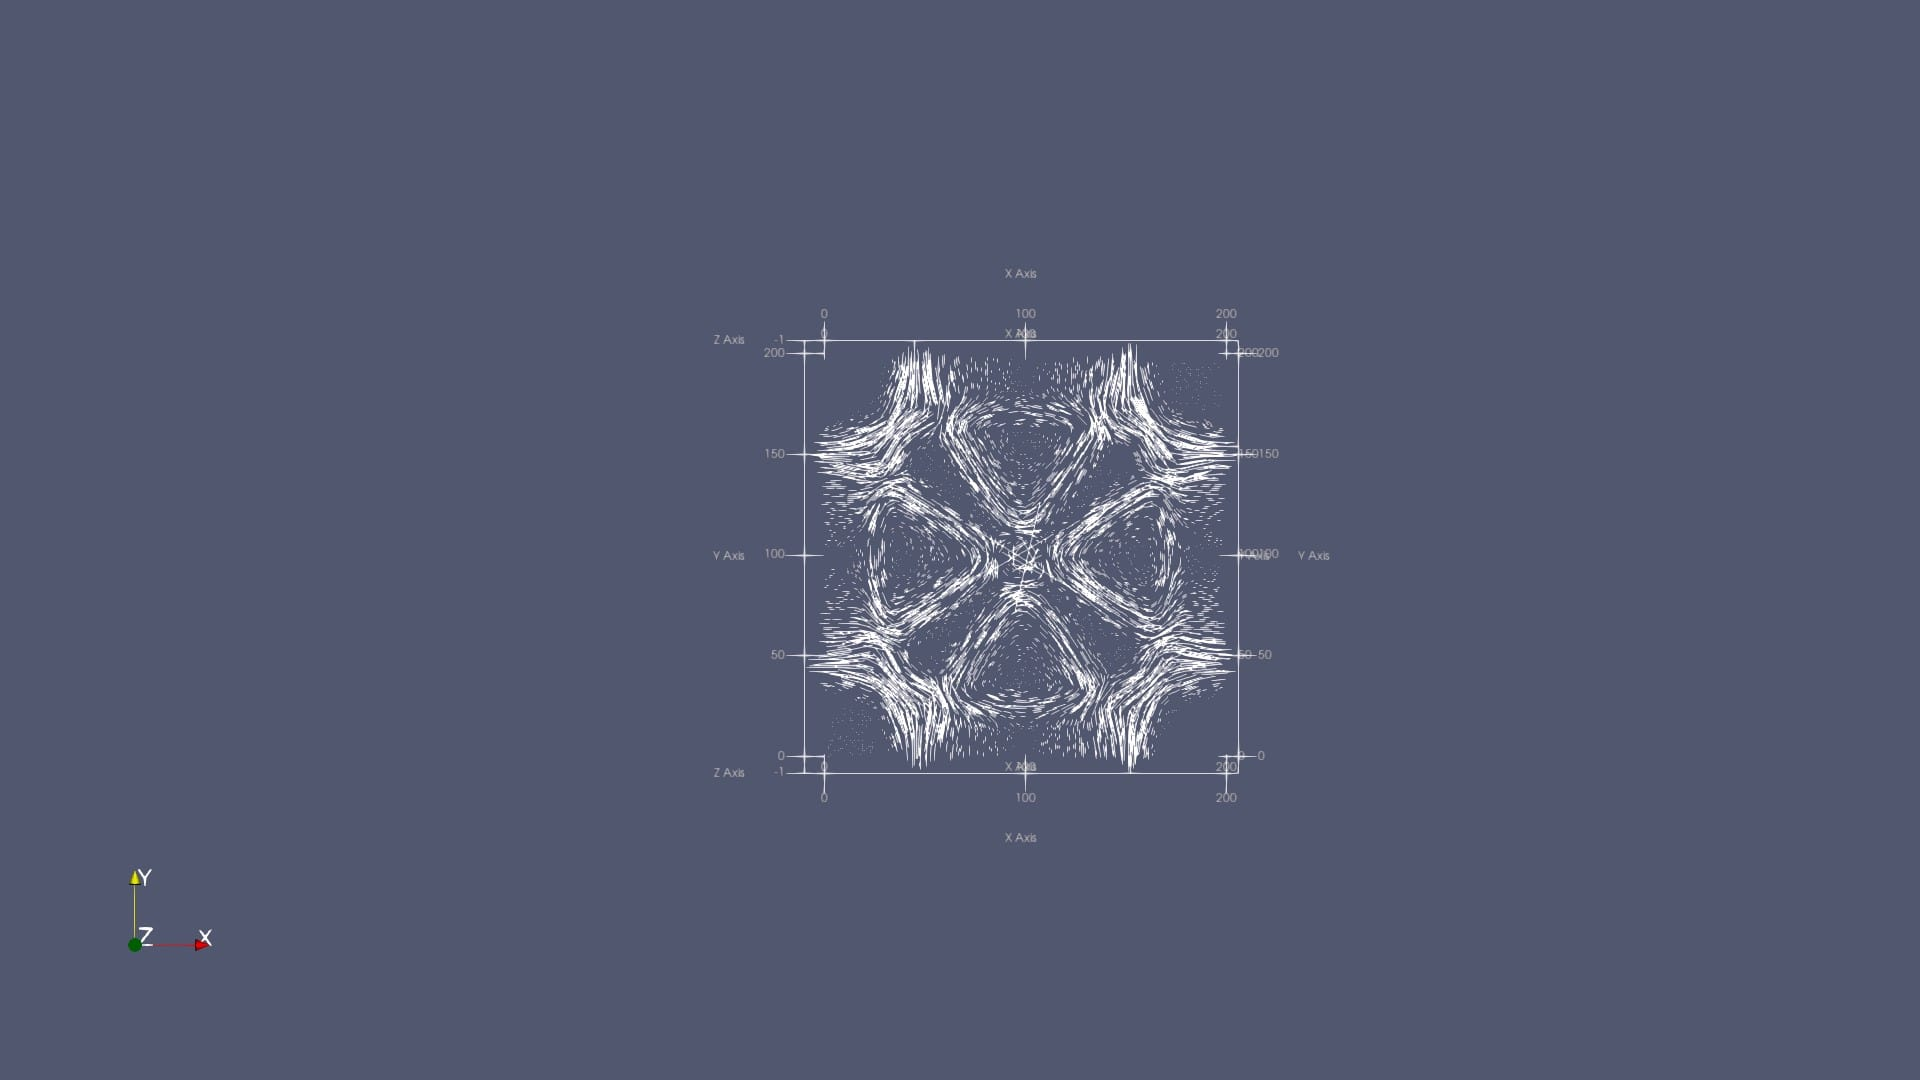
\includegraphics[width=.95\linewidth]{Figures/FDTD2DE2}
    	\caption{t = 400}
    \end{subfigure}
    \begin{subfigure}{.49\textwidth}
    	\centering
    	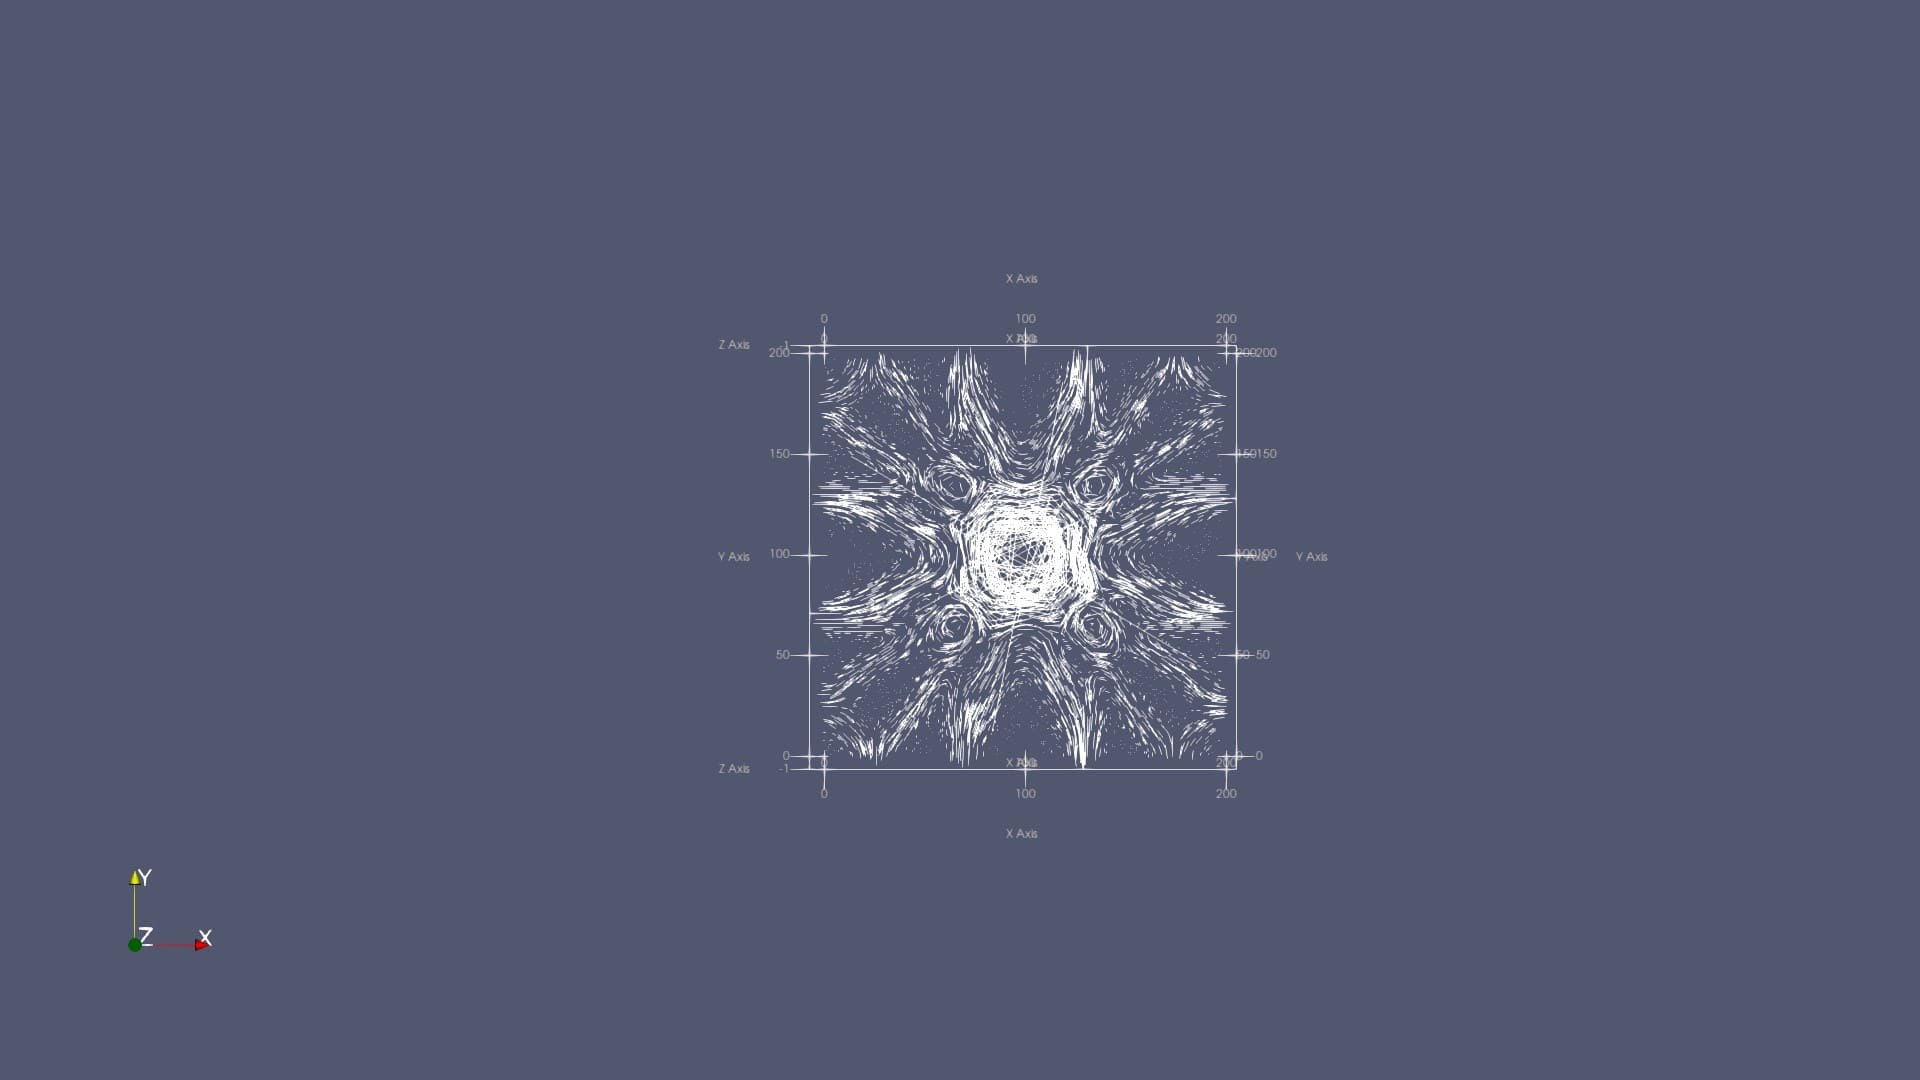
\includegraphics[width=.95\linewidth]{Figures/FDTD2DE3}
    	\caption{t = 600}
    \end{subfigure}
    \begin{subfigure}{.49\textwidth}
    	\centering
    	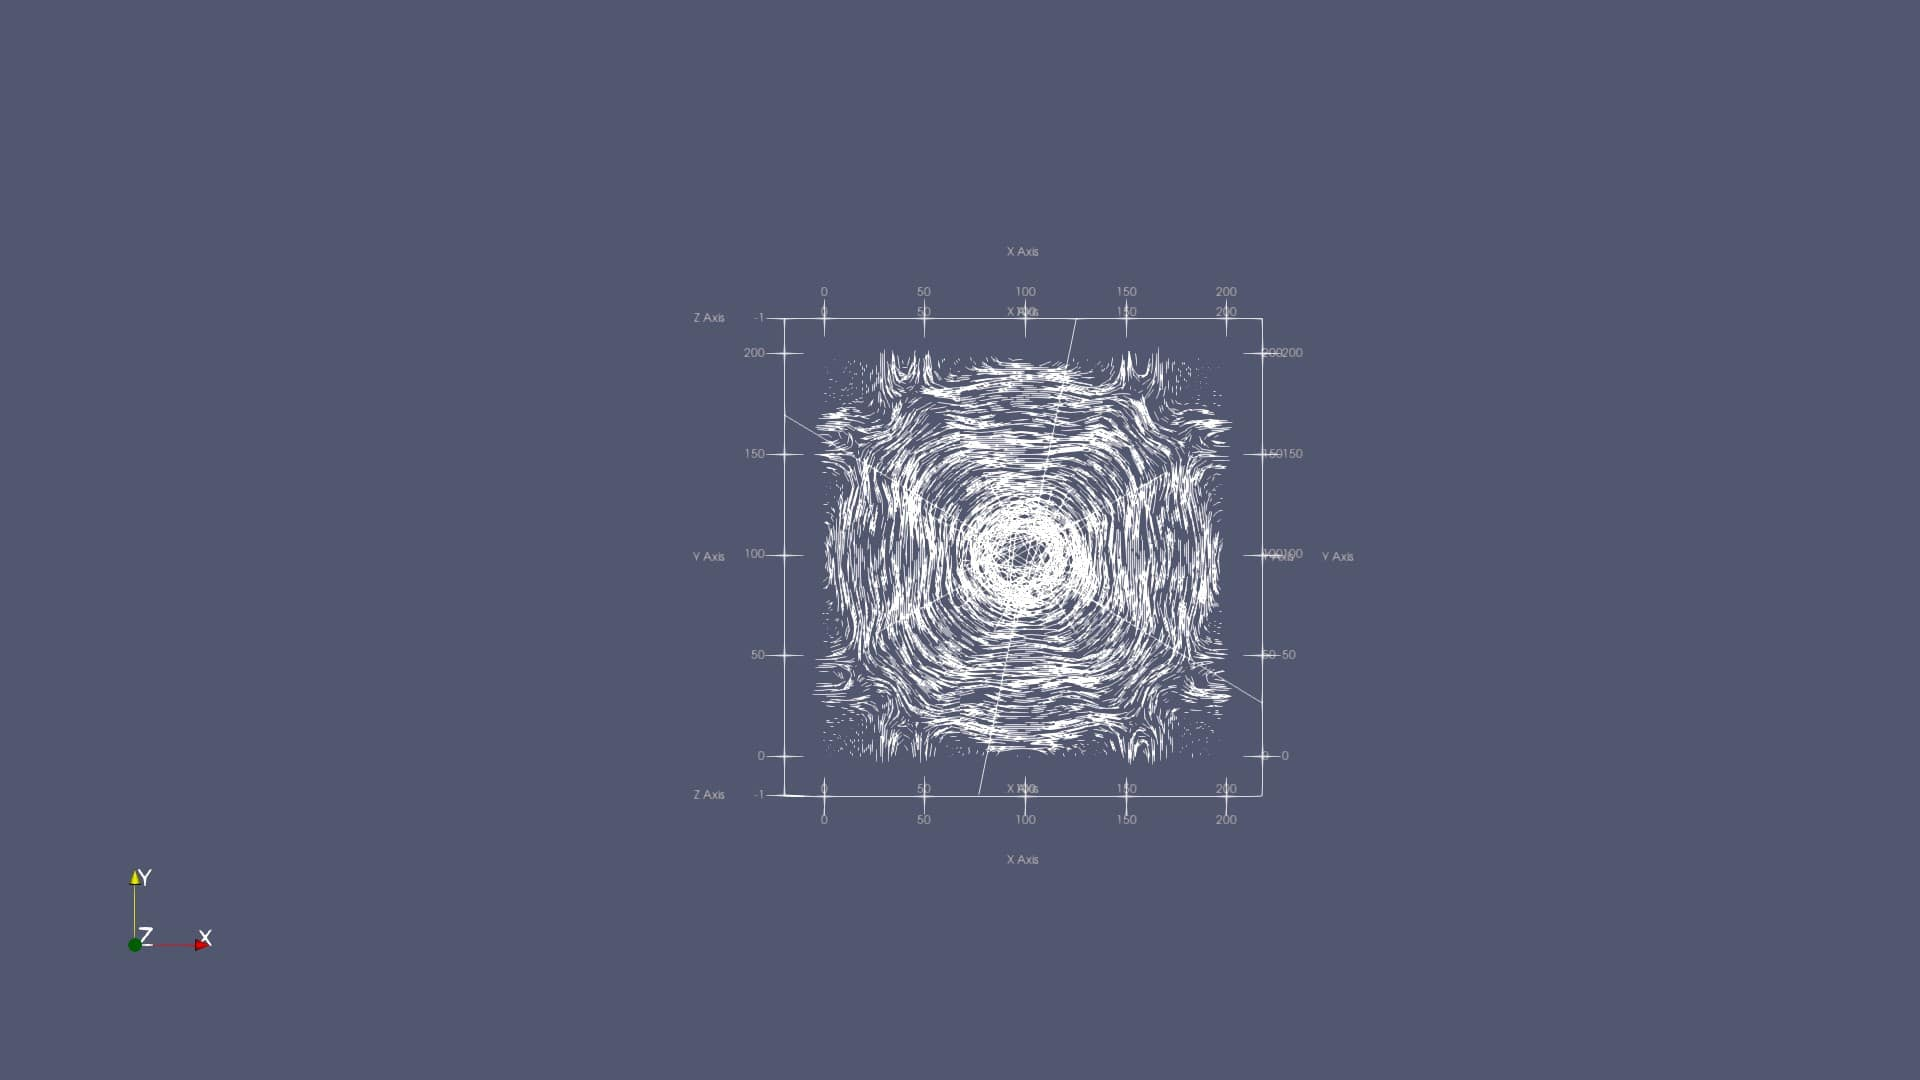
\includegraphics[width=.95\linewidth]{Figures/FDTD2DE4}
    	\caption{t = 800}
    \end{subfigure}
	\decoRule
	\caption[2D Electric Field Simulation]{A simulation of the 2D electric field.}
	\label{fig:FDTD2DE}
\end{figure}

The above is for the electric data. For the magnetic data we can use a simple \textbf{Table to Structured Grid}, and it will be good just like that. With a few adjustments to colors and scaling, we can achieve the following result (Figure \ref{fig:FDTD2DH}):

\begin{figure}[h!]
	\centering
	\begin{subfigure}{.49\textwidth}
		\centering
		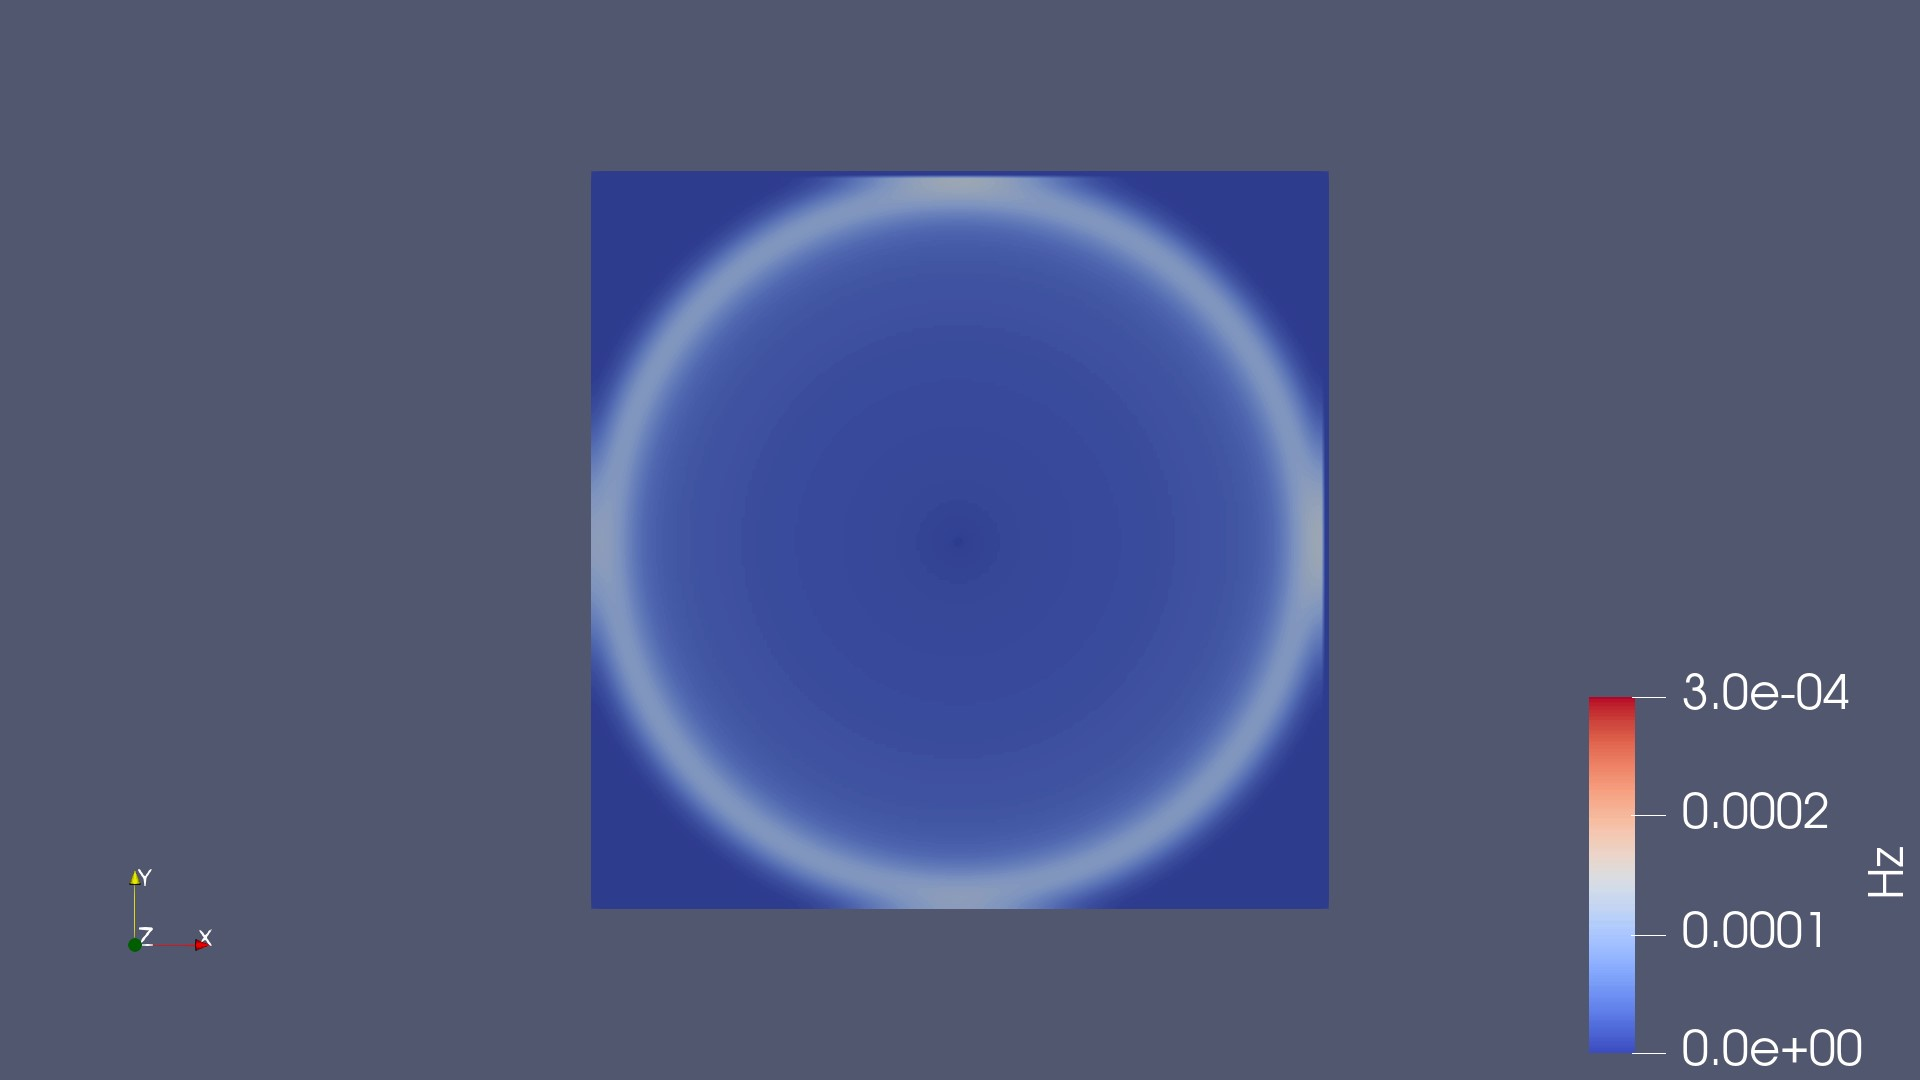
\includegraphics[width=.95\linewidth]{Figures/FDTD2DH1}
		\caption{t = 200}
	\end{subfigure}
	\begin{subfigure}{.49\textwidth}
		\centering
		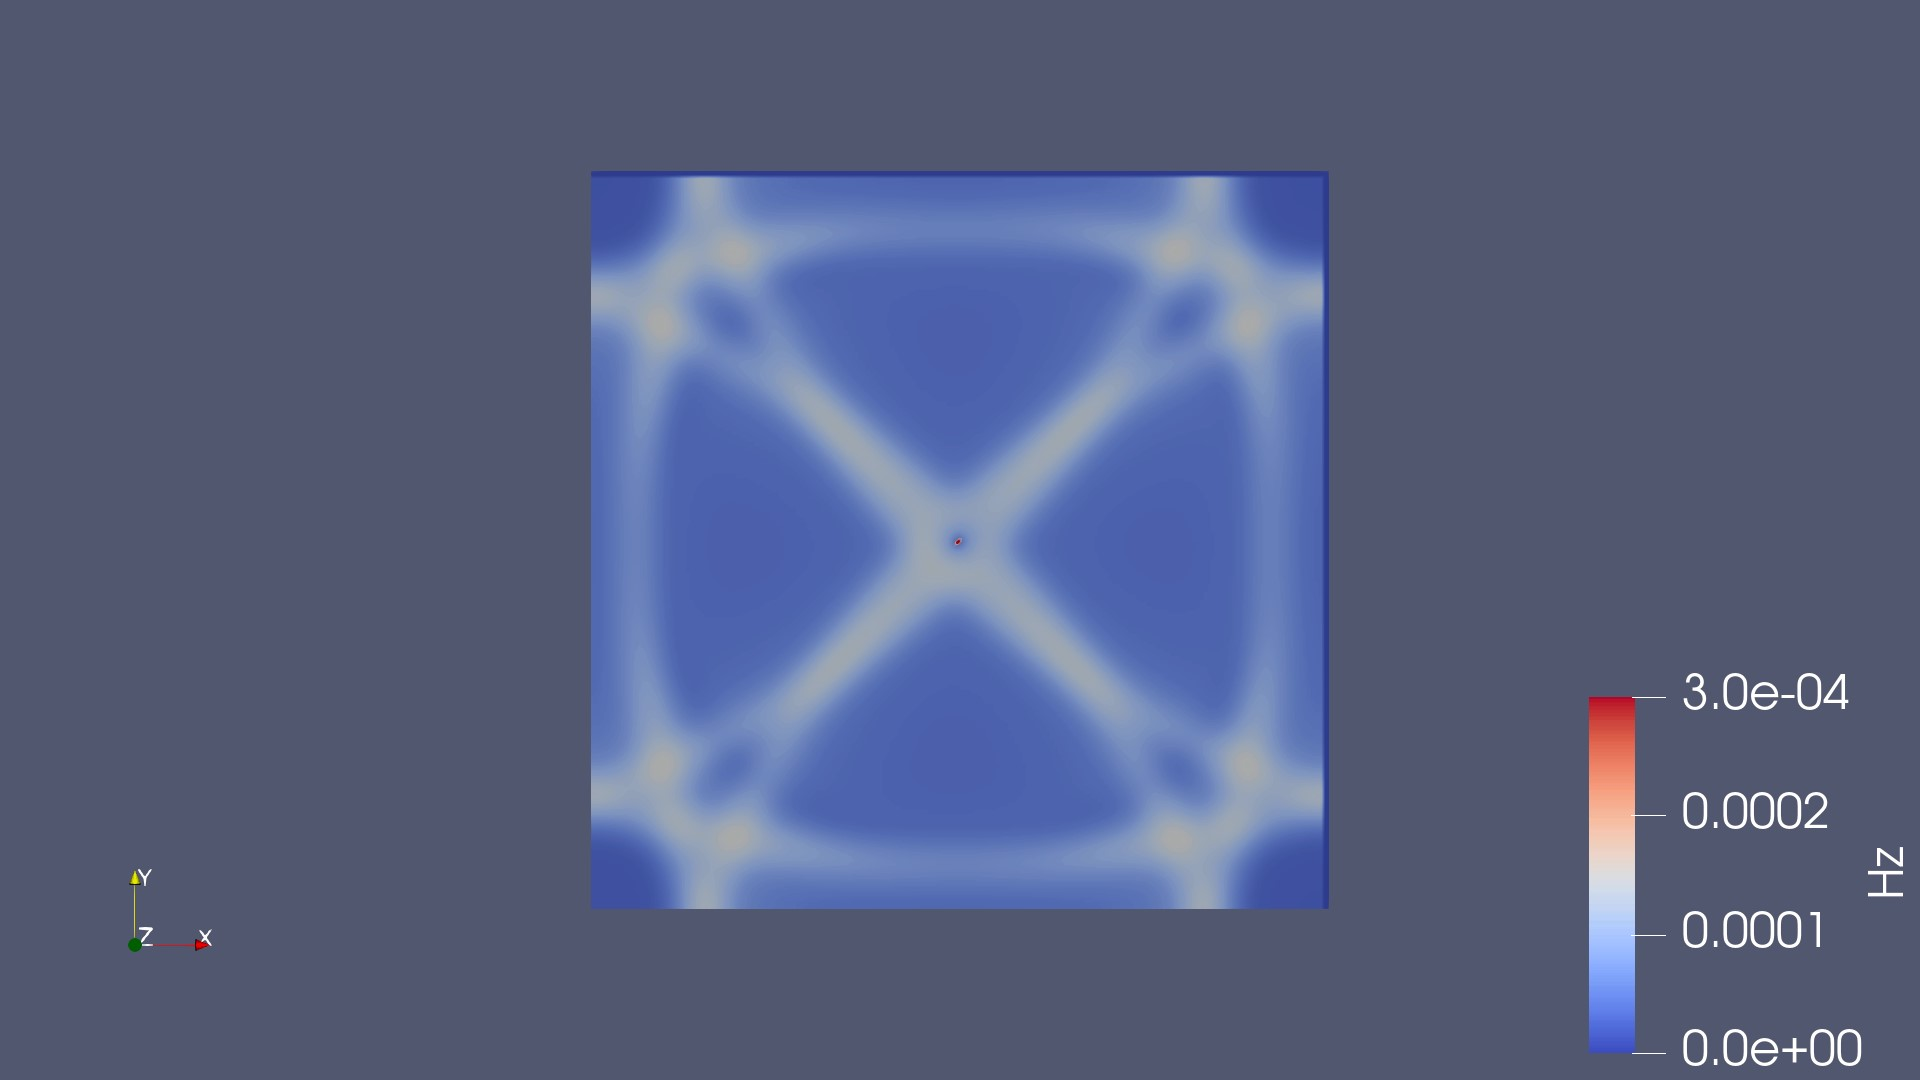
\includegraphics[width=.95\linewidth]{Figures/FDTD2DH2}
		\caption{t = 400}
	\end{subfigure}
	\begin{subfigure}{.49\textwidth}
		\centering
		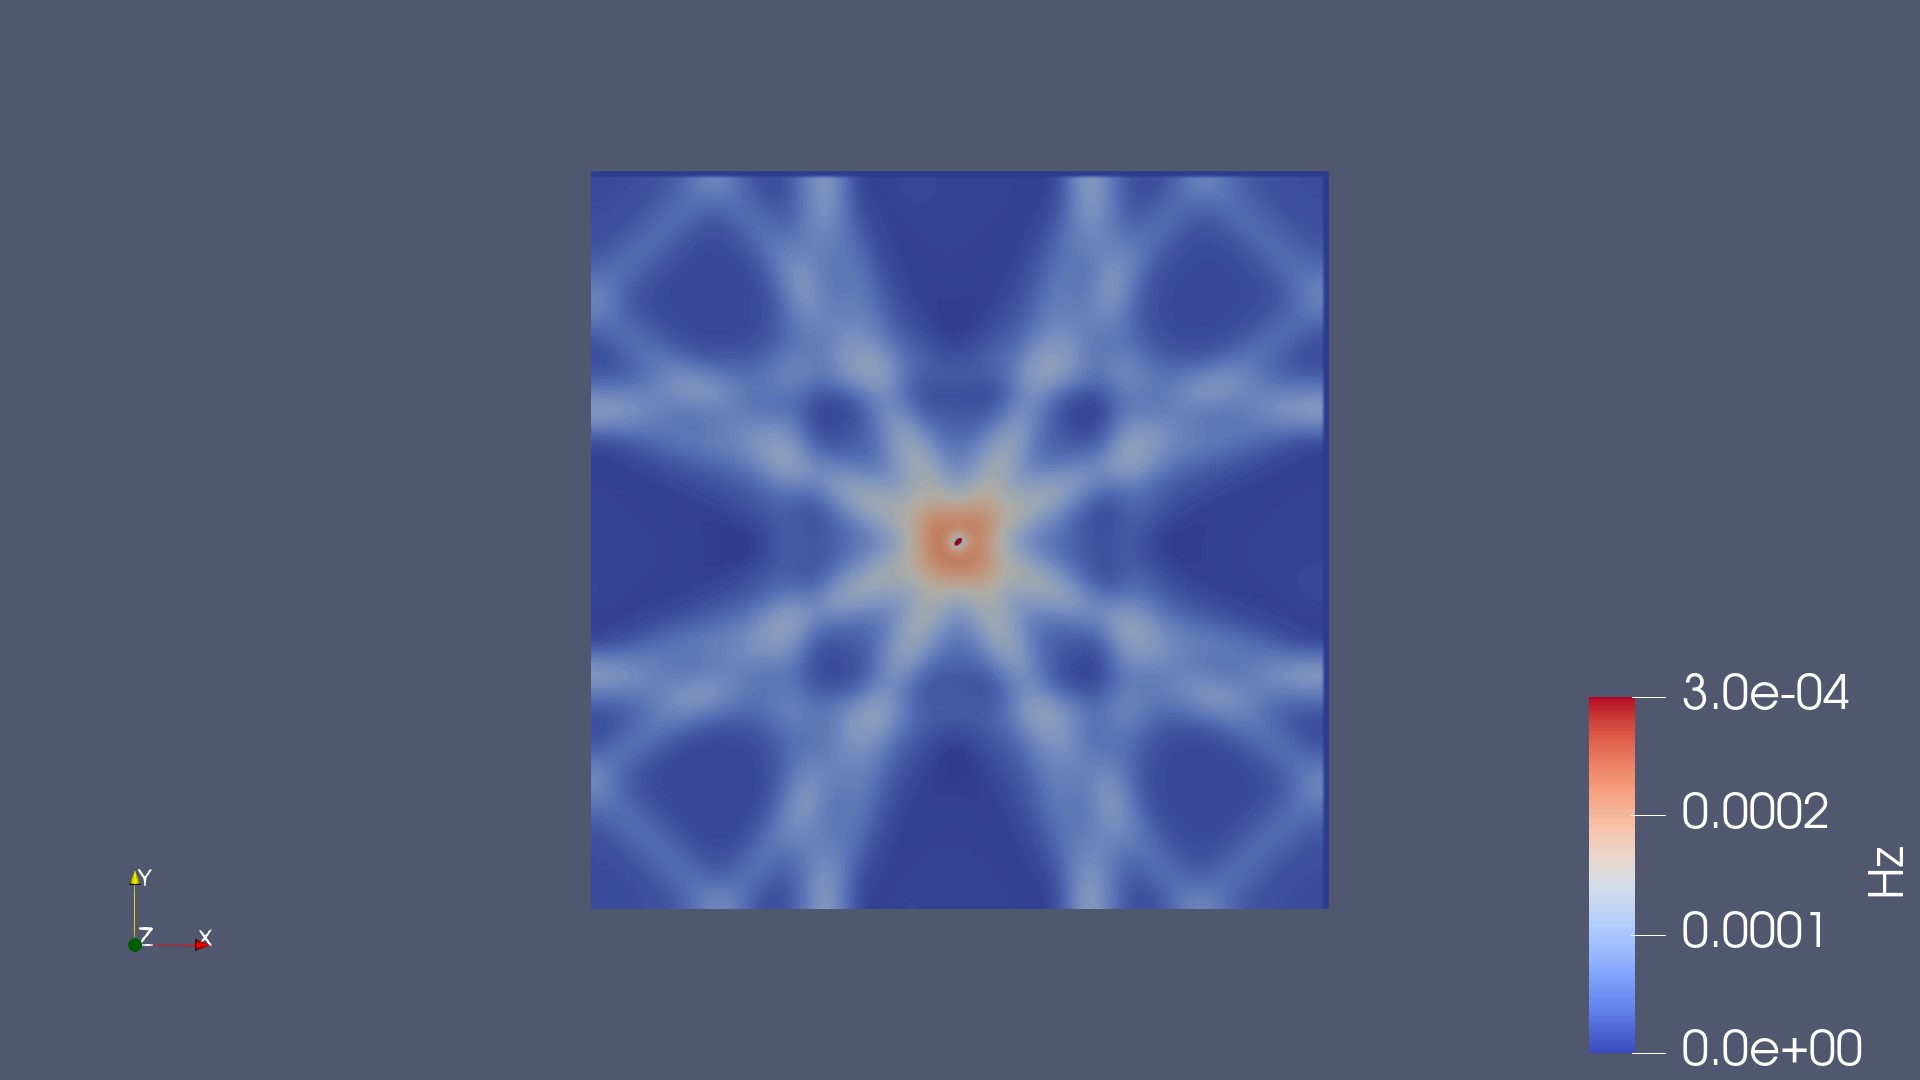
\includegraphics[width=.95\linewidth]{Figures/FDTD2DH3}
		\caption{t = 600}
	\end{subfigure}
	\begin{subfigure}{.49\textwidth}
		\centering
		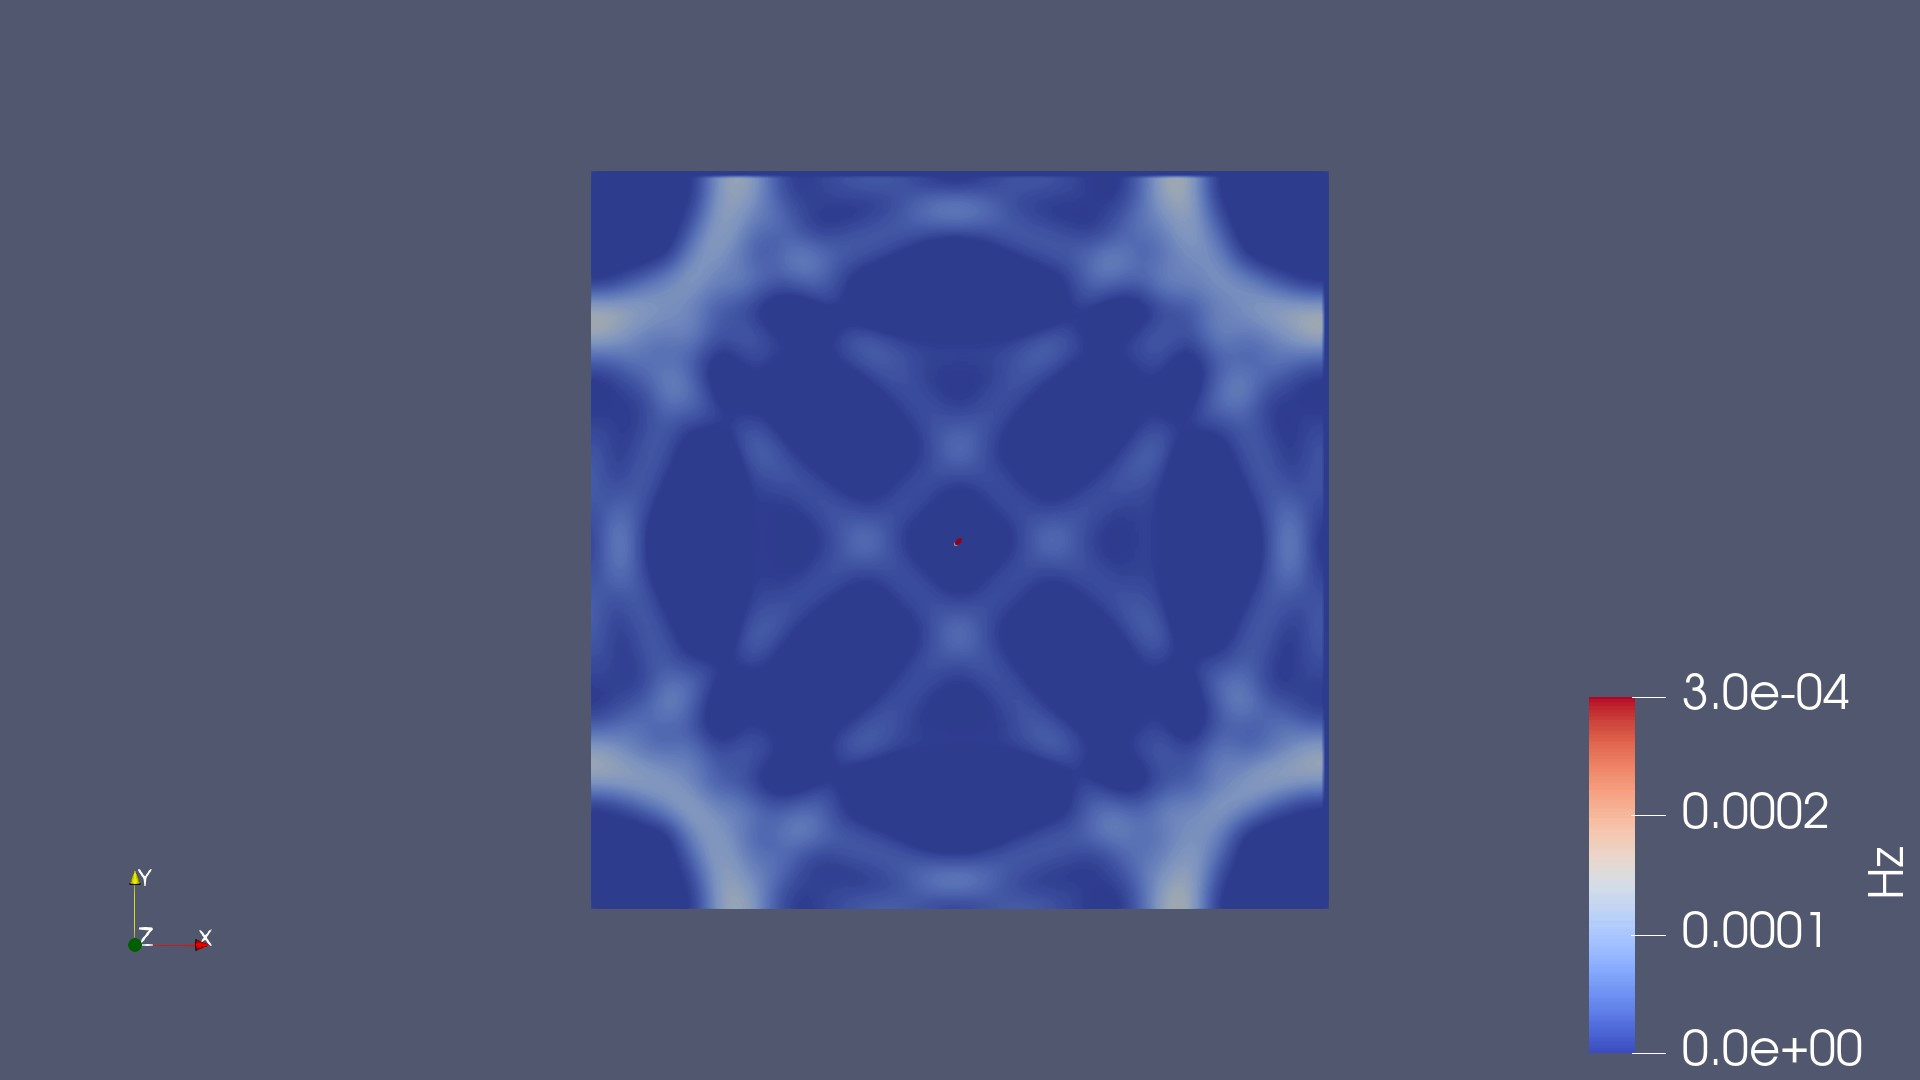
\includegraphics[width=.95\linewidth]{Figures/FDTD2DH4}
		\caption{t = 800}
	\end{subfigure}
	\decoRule
	\caption[2D Magnetic Field Simulation]{A simulation of the 2D magnetic field.}
	\label{fig:FDTD2DH}
\end{figure}

Moving forward, we are going to use only the method we used for visualizing electric field data, as the \textbf{Table to Structured Grid} method is not usable when we use more than one vector. With that done, we can finally move on to the three-dimensional scenario, which is the most useful one for practical real life applications.